\documentclass[12pt,a4paper]{report}
\usepackage[utf8]{inputenc}
\usepackage{amsmath}
\usepackage{amsfonts}
\usepackage{amssymb}
\usepackage{makeidx}
\usepackage{graphicx}
\usepackage{algorithm,listings}
\usepackage{algpseudocode}

\newcommand{\mytitle}{AIDRA: AI-based Diagnosis using RAG Architecture}
\newcommand{\titleKey}{AIDRA}


\usepackage[left=4cm,right=2cm,top=3cm,bottom=3cm]{geometry}
\newcommand{\mySpace}{0.5cm}
\newcommand{\mySpaceHalf}{0.5cm}
\usepackage{tikz}
\usetikzlibrary{shapes,arrows,positioning}
\renewcommand{\contentsname}{\centering Contents}
\usepackage{hyperref}


\begin{document}
\clearpage
	\newgeometry{left=2cm, right=2cm, top=3cm, bottom=3cm}
	\begin{titlepage}

    \centering
    %{\Huge \mytitle \fontsize{24}{28.8}\selectfont
     %\fontfamily{ptm}\selectfont}\\

{\Huge  \textmd{ AIDRA \\[0.5cm] \textit{AI-based Diagnosis using RAG Architecture}} \fontsize{24}{28.8}\selectfont 
\fontfamily{ptm}\selectfont}\\


%{\Huge AIDRA\\[0.5cm](AI-based Diagnosis using RAG Architecture) \fontsize{24}{28.8}\selectfont 
%\fontfamily{ptm}\selectfont}\\

%\fontsize{24}{10}\selectfont \textbf{ AIDRA \\[0.5cm] AI-based Diagnosis using RAG Architecture}

    
\vspace{\mySpace}
%	\begin{center}
 %   		{\fontsize{24}{28.8}\selectfont  {Gesture-Nav: Hand-Controlled Virtual Mouse}}
%	\end{center}
    \large \textit{By}\\
\vspace{\mySpace}
    {\Large AVISHEK MONDAL ( CSE21019 / 679 )  \\
    \vspace{0.11cm}
    SOUVIK BAIDYA ( CSE21088  / 748 )\\
    \vspace{0.11cm}
    TAMAL MALLICK ( CSE21099 / 759 ) \\
    \fontsize{18}{22}\selectfont \fontfamily{ptm}\selectfont
\vspace{\mySpace}}
    \begin{center}
        
\includegraphics[width=0.5\textwidth]{iiitk_logo} %img
    \end{center}
    {\Large \textit{Bachelor Thesis submitted to}\\
    \vspace{\mySpaceHalf}
    Indian Institute of Information Technology Kalyani \\ \vspace{\mySpaceHalf}
	 \textit{for the partial fulfillment of the degree of}\\ \vspace{\mySpaceHalf}

{\bfseries %bolding
	 Bachelor of Technology \\ 
	 in \\
	 Computer Science and Engineering\\ \vspace{\mySpaceHalf}
	  May, 2025 \fontsize{18}{22}}\selectfont \fontfamily{ptm}\selectfont}
    \vspace*{\fill}
\end{titlepage}
\restoregeometry


%	\author{Tamal Mallick , Avishek Mondal, Souvik Baidya}
%	\title{GestureNav: Hand-Controlled Virtual Mouse }
%	\maketitle
%	GestureNav: Hand Controlled Virtual Mouse
%
	\newpage
	\pagenumbering{roman}
	\chapter*{\centering Certificate}
\label{sec:engack}
This is to certify that the synopsis entitled \textbf{"\mytitle "} is being submitted by Tamal Mallick,
 (\textbf{Enrollment No: CSE/21099/759 }), Avishek Mondal (\textbf{Enrollment No: CSE21019/679}) and Souvik Baidya (\textbf{Enrollment No: CSE21088/748}), B.Tech., Indian Institute of Information Technology Kalyani, India, for the partial fulfillment of the requirements for the registration of the degree of Bachelor of Technology is an original research work carried by them under my supervision. The synopsis has fulfilled all the requirements as per the regulation of IIIT Kalyani and in my opinion, has reached the standards needed for submission. The works, techniques, and results presented have not been submitted to any other university or Institute for the award of any other degree or diploma.
\\
\\
\\
\\
\\
\\
\\
\\
\noindent
\textbf{Dr. Anirban Lakshman}  \\ 
\textit{Assistant Professor \\
Department of Mathematics\\
Indian Institute of Information Technology Kalyani \\
Kalyani - 741235, W.B., India.} \\[1em]
%$Assistant Professor \\  
%Department of Mathematics\\
%Indian Institute of Information Technology Kalyani\\
%Kalyani-741235, W.B., India.
%$
\cleardoublepage



	\chapter*{\centering Declaration}
\label{sec:engack}
We hereby declare that the work being submitted in this thesis entitled,\textbf{"\mytitle "}, submitted to Indian Institute of Information Technology, Kalyani in partial fulfillment for the award of the degree of Bachelor of Technology in Computer Science and Engineering during the period from July, 2024 to November 2024 under the supervision of Dr. Anirban Lakshman, Department of Computer Science and Engineering, Indian Institute of Information Technology Kalyani, West Bengal 741235, India, does not contain any classified information. 
\\
\\
\\
\\
\\
\\
\\
\noindent
\textbf{Tamal Mallick} \\
\textit{Enrollment No.: CSE/21099/759 \\
Indian Institute of Information Technology Kalyani \\
Kalyani - 741235, W.B., India.} \\[1em]
\\[1.2cm]
\noindent
\textbf{Avishek Mondal} \\
\textit{Enrollment No.: CSE/21019/679 \\
Indian Institute of Information Technology Kalyani \\
Kalyani - 741235, W.B., India.} \\[1em]
\\[1.2cm]
\noindent
\textbf{Souvik Baidya} \\
\textit{Enrollment No.: CSE21088/748 \\
Indian Institute of Information Technology Kalyani \\
Kalyani - 741235, W.B., India.}

\cleardoublepage
	
			\newpage
			\chapter*{\centering Acknowledgement}
We hereby acknowledge our deep sense of gratitude to our supervisor \textbf{Dr. Anirban Lakshman}, Department of Mathematics, Indian Institute of Information Technology Kalyani, for providing us with adequate facilities, ways, and means by which we are able to do this work. We express our sincere gratitude to him, his valuable time, insightful suggestions, and constant support have been indispensable for our progress.\\
\\
	Finally, we would also like to thank our friends, college faculties and family members who in one way or another helped us in doing this work.\\
\\
\\
\\
\\
\\
\noindent
\textbf{Tamal Mallick} \\
\textit{Enrollment No.: CSE/21099/759 \\
Indian Institute of Information Technology Kalyani \\
Kalyani - 741235, W.B., India.} \\[1em]
\\[1.2cm]
\noindent
\textbf{Avishek Mondal} \\
\textit{Enrollment No.: CSE/21019/679 \\
Indian Institute of Information Technology Kalyani \\
Kalyani - 741235, W.B., India.} \\[1em]
\\[1.2cm]
\noindent
\textbf{Souvik Baidya} \\
\textit{Enrollment No.: CSE21088/748 \\
Indian Institute of Information Technology Kalyani \\
Kalyani - 741235, W.B., India.}


\cleardoublepage
\chapter*{\centering Abstract}
\label{Abstract}

This project, entitled \textbf{"\mytitle"}, presents the development of an intelligent medical chatbot designed to assist users with accurate and trustworthy health-related information. Unlike traditional chatbots or wellness assistants focused solely on general advice or alternative therapies, this system leverages state-of-the-art Large Language Models (LLMs) integrated with Retrieval-Augmented Generation (RAG) to deliver context-aware, medically accurate responses \cite{chatgpt, langchain}.

The chatbot sources its information from globally respected clinical references such as the \textit{Oxford Handbook of Clinical Medicine}, \textit{Harrison’s Principles of Internal Medicine}, and \textit{The Merck Manual} (referenced in the indexed dataset, not explicitly cited here due to lack of publication detail in your `.bib`). 

The core functionalities of the chatbot include analyzing user-described symptoms, suggesting relevant diagnostic tests, identifying possible conditions, and recommending appropriate medications when a confident match is found in the context. It also provides lifestyle and dietary advice tailored to specific conditions. To ensure efficient and relevant information retrieval, the project utilizes HuggingFace embeddings \cite{sentence_transformers} and the Pinecone vector database \cite{pinecone}, managed through the LangChain framework \cite{langchain}. The system is deployed via a Flask web interface, offering users an interactive and responsive experience.

By combining trusted medical literature with advanced natural language processing, the chatbot aims to simulate the reasoning of a professional physician in non-critical scenarios, empowering users with reliable medical insights while clearly avoiding emergency diagnosis use cases.





\cleardoublepage



		\tableofcontents

			\chapter*{\centering Abbreviations Used }
		\label{Abbreviations Used}
		
		

\begin{table}[ht]
\centering
\begin{tabular}{|c|l|}
\hline
\textbf{Abbreviation} & \textbf{Full Form} \\ \hline

\multicolumn{2}{|c|}{\textbf{Artificial Intelligence and Machine Learning}} \\ \hline
RAG & Retrieval-Augmented Generation \\ \hline
LLM & Large Language Model \\ \hline
STT & Speech-to-Text \\ \hline
TTS & Text-to-Speech \\ \hline
ML & Machine Learning \\ \hline
AI & Artificial Intelligence \\ \hline
NLP & Natural Language Processing \\ \hline
MLOps & Machine Learning Operations \\ \hline

\multicolumn{2}{|c|}{\textbf{General Healthcare}} \\ \hline
FPG & Fasting Plasma Glucose \\ \hline
HbA1c & Hemoglobin A1c \\ \hline
CT & Computed Tomography \\ \hline
eGFR & Estimated Glomerular Filtration Rate \\ \hline
KUB & Kidneys, Ureters, and Bladder X-ray \\ \hline
MRI & Magnetic Resonance Imaging \\ \hline
WGS & Whole Genome Sequencing \\ \hline
CBC & Complete Blood Count \\ \hline
WHO & World Health Organization \\ \hline
CDC & Centers for Disease Control and Prevention \\ \hline


\multicolumn{2}{|c|}{\textbf{Technology and Infrastructure}} \\ \hline
API & Application Programming Interface \\ \hline
GUI & Graphical User Interface \\ \hline
VM & Virtual Machine \\ \hline
SSL & Secure Sockets Layer \\ \hline
DB & Database \\ \hline
DevOps & Development and Operations \\ \hline

\end{tabular}
\caption{List of Abbreviations Used in the Project}
\label{tab:abbreviations}
\end{table}






	\renewcommand{\thesection}{\arabic{section}}
	
	\newpage
		\pagenumbering{arabic}
	{\vfill \chapter*{\centering \vfill Chapter 1 \vfill}\vfill}
	\thispagestyle{empty}
	\newpage

	\label{Introduction}
	\section{Introduction}

	\label{Background}
	\subsection{Background }
The use of AI-driven chatbots in the healthcare domain is evolving rapidly, particularly with the advent of advanced large language models (LLMs). These models are capable of understanding and generating human-like responses, making them suitable for developing conversational agents. However, traditional healthcare chatbots have limitations in personalization, adaptability, and factual accuracy, especially in niche domains like alternative medicine. The concept of Retrieval-Augmented Generation (RAG) offers a promising solution by enriching LLMs with real-world knowledge from curated sources. This project, titled \textbf{\titleKey} leverages RAG to deliver a chatbot capable of answering user queries in the field of holistic and alternative medicine.`


\label{Motivation}  
\subsection{Motivation}  

Access to \textbf{quality healthcare} remains a \textbf{critical challenge} in many parts of the world. According to global health reports, at least \textbf{half of the population} lacks access to essential health services \cite{worldbank_who}. Moreover, over \textbf{1 billion people} are pushed into extreme poverty annually due to \textbf{out-of-pocket medical expenses}, especially in low- and middle-income countries \cite{worldbank_who} .

In countries like \textbf{India}, approximately \textbf{55 million people} fall below the poverty line each year due to unaffordable healthcare \cite{phfi}. Even for \textbf{minor but untreated medical conditions}, the lack of timely consultation often leads to \textbf{severe complications or even death}.

Additionally, it is reported that \textbf{2.6 million people} die annually as a result of \textbf{unsafe medical practices} \cite{who_patientsafety}. A significant portion of these deaths could be prevented if \textbf{reliable and early medical advice} were accessible to all.

While \textbf{AI-based solutions} are increasingly being used in healthcare, most \textbf{generic chatbots hallucinate} or provide \textbf{inaccurate information}, especially when queried for \textbf{specialized medical advice}. This motivated the development of a \textbf{Retrieval-Augmented Generation (RAG)-based Medical Chatbot}, which we have named the \textbf{\titleKey}. Our chatbot utilizes trusted medical references like \textit{Harrison's Principles of Internal Medicine}, the \textit{Oxford Handbook of Clinical Medicine}, and the \textit{Merck Manual}, to ensure that the information it provides is \textbf{credible, contextual, and verifiable}.

This project aims to \textbf{democratize access} to trustworthy medical knowledge, especially for those who \textbf{cannot afford quality healthcare}, by providing \textbf{symptom-based diagnosis support}, \textbf{test suggestions}, and \textbf{prescription-level medical guidance} powered by \textbf{reliable clinical sources}.




\title{Problem Statement}
\subsection{Problem Statement}  
Despite their linguistic capabilities, general-purpose \textbf{large language models (LLMs)} struggle to offer \textbf{domain-specific}, context-aware, and explainable medical advice. These models often respond with \textbf{hallucinated outputs} that may seem convincing but are not grounded in verified clinical data.

This limitation poses a significant risk in the medical field, where \textbf{accuracy}, \textbf{safety}, and source \textbf{verifiability} are non-negotiable. Furthermore, these models typically do not offer \textbf{traceability} of their responses, making it difficult for users to trust or validate the suggestions.

The challenge lies in building a chatbot system that:
\begin{itemize}
  \item Can retrieve \textbf{real-time relevant content} from a trusted medical database;
  \item Contextualizes the patient’s input (symptoms, test reports, etc.) before generating a response;
  \item Prescribes medications or suggests medical tests only when backed by \textbf{validated medical sources}.
\end{itemize}

Our solution, \titleKey, combines \textbf{retrieval-augmented generation} techniques with advanced LLMs to simulate the behavior of a virtual medical assistant. By leveraging a \textbf{vector database} for storing and querying reliable medical knowledge, the system ensures that its recommendations are grounded in \textbf{evidence} and \textbf{transparent} to the user.
 
 
 
\title{Objectives}
\subsection{Objectives}  
The primary goal of this project is to build an intelligent medical assistant that delivers reliable, context-aware, and explainable healthcare guidance.

\begin{itemize}
    \item To create an \textbf{LLM-powered virtual medical specialist} capable of providing \textbf{reliable medication suggestions and prescriptions} based on trusted sources.
    
    \item To design a chatbot that utilizes \textbf{Retrieval-Augmented Generation (RAG)} to ensure \textbf{higher response accuracy} and \textbf{contextual relevance}.
    
    \item To integrate \textbf{LangChain}, \textbf{Gemini LLM}, and \textbf{Pinecone} into a complete \textbf{retrieval and generation pipeline} for intelligent medical dialogue.
    
    \item To provide users with a \textbf{simple and intuitive interface} for querying holistic and modern medical content.
    
    \item To ground all responses using a \textbf{curated dataset} derived from world-renowned medical references, including the \textit{Gale Encyclopedia of Alternative Medicine}, the \textit{Oxford Handbook of Clinical Medicine}, \textit{Harrison’s Principles of Internal Medicine}, and \textit{The Merck Manual}.
\end{itemize}




\title{Scope of Work}
\subsection{Scope of Work}

\subsubsection*{Functional Scope}

The medical chatbot is designed to deliver \textbf{intelligent}, \textbf{context-aware responses} to user health-related queries. Its scope extends beyond general wellness or alternative therapies, offering \textbf{clinically grounded guidance}, including potential diagnoses, diagnostic test recommendations, and medication suggestions based on trusted clinical literature like the \textit{Oxford Handbook of Clinical Medicine}, \textit{Harrison’s Principles of Internal Medicine}, and \textit{The Merck Manual}.

While the system is \textbf{not intended for emergency use or life-threatening conditions}, it aims to simulate the reasoning and response behavior of a \textbf{professional doctor} in non-critical scenarios. The chatbot can:

\begin{itemize}
    \item Analyze user-described \textbf{symptoms},
    \item Suggest relevant \textbf{diagnostic tests},
    \item Propose possible \textbf{conditions or diseases},
    \item Recommend \textbf{medications} (only when confidence is high and backed by context),
    \item Provide \textbf{dietary and lifestyle advice} related to the diagnosed or suspected condition.
\end{itemize}

\subsubsection*{Technical Scope}

The technical components that define the system include:

\begin{itemize}
    \item \textbf{Document ingestion and preprocessing},
    \item \textbf{Embedding generation and vector storage} using Pinecone,
    \item Implementation of \textbf{Retrieval-Augmented Generation (RAG)} with LangChain,
    \item Development of a \textbf{custom contextual memory system},
    \item \textbf{Prompt engineering} to enforce structured, medically accurate outputs,
    \item \textbf{Web deployment} via a Flask-based interface for end-user interaction.
\end{itemize}





	{\vfill \chapter*{\centering \vfill Chapter 2 \vfill}\vfill}
	\thispagestyle{empty}
	\newpage
\section{Literature Review}
\label{Literature Review}

This section presents a review of existing systems and research in the field of AI-driven medical chatbots, with a focus on their capabilities, limitations, and relevance to the development of the \titleKey{} system. It explores advancements in healthcare chatbots, generative AI models, and the integration of Retrieval-Augmented Generation (RAG) with vector databases. The review also includes a discussion on prompt engineering practices that help ensure medically accurate, trustworthy, and explainable outputs in conversational healthcare applications.

\subsection{Existing Chatbots in Healthcare}
\label{subsec:existing-chatbots}

Several healthcare chatbots, such as \textbf{Ada Health}, \textbf{Babylon Health}, and \textbf{HealthTap}, are widely used in digital healthcare \cite{digital_health_platforms}. These platforms primarily focus on \textbf{symptom analysis} and \textbf{rule-based triage} using structured datasets. While they are effective for \textbf{basic diagnostics}, their \textbf{general-purpose architecture} limits adaptability to \textbf{complex or domain-specific applications}, such as medically grounded prescription generation or handling of alternative therapies.

\subsection{Generative AI and Medical Applications}
\label{subsec:generative-ai-medical}

Recent advancements in \textbf{Generative AI} models like \textbf{ChatGPT} (OpenAI), \textbf{Bard} (Google), and \textbf{Claude} (Anthropic) have shown remarkable progress in \textbf{natural language understanding} and \textbf{response generation}. However, these models often lack \textbf{domain grounding}, leading to \textbf{speculative or inaccurate responses} when queried for medical advice \cite{chatgpt, hallucination_survey}. In healthcare applications, \textbf{factual correctness}, \textbf{explainability}, and \textbf{source traceability} are critical — which general LLMs often fail to consistently deliver.

\subsection{Retrieval-Augmented Generation (RAG)}
\label{subsec:rag}

\textbf{Retrieval-Augmented Generation (RAG)} is a paradigm that enhances LLM performance by combining \textbf{document retrieval} with \textbf{generative response} \cite{langchain}. Instead of depending solely on the model's internal parameters, RAG retrieves relevant context documents from a \textbf{vector store}, ensuring that outputs are \textbf{context-aware} and \textbf{factually grounded}. \textbf{LangChain}, a Python framework used in this project, simplifies this integration by offering modular components for \textbf{document loading}, \textbf{chunking}, \textbf{embedding}, \textbf{retrieval}, and \textbf{LLM orchestration} \cite{langchain}.

\subsection{Embedding Models and Vector Databases}
\label{subsec:embeddings-vectors}

This project uses \textbf{HuggingFace’s all-MiniLM-L6-v2}, a transformer-based sentence embedding model that captures \textbf{semantic similarity} between texts \cite{sentence_transformers}. These embeddings are indexed in \textbf{Pinecone}, a high-speed, scalable vector database, allowing efficient \textbf{semantic search} to retrieve relevant chunks during inference \cite{pinecone}. This architecture forms the backbone of the \titleKey{} system, enabling reliable information grounding.

\subsection{Prompt Engineering}
\label{subsec:prompt-engineering}

\textbf{Prompt engineering} is pivotal for customizing LLM outputs in task-specific scenarios. In this project, a carefully crafted prompt instructs the \textbf{Gemini LLM} to behave like a professional doctor, \textbf{Dr. Sushruta}, drawing information only from trusted medical references. The prompt format ensures that answers are \textbf{context-restricted}, \textbf{medically relevant}, and delivered in a \textbf{structured JSON format}. This approach helps \textbf{minimize hallucination} and encourages \textbf{clinically appropriate response behavior} \cite{hallucination_survey}.






	{\vfill \chapter*{\centering \vfill Chapter 3 \vfill}\vfill}
	\thispagestyle{empty}
	\newpage
	\label{System Design and Architecture}
	\section{System Design and Architecture}
	\label{Workflow Overview}
	\subsection{Workflow Overview}

The architecture of \titleKey{} is designed around a modular\\ \textbf{Retrieval-Augmented Generation (RAG)} pipeline. Each component is independently structured to allow for \textbf{debugging}, \textbf{modular development}, and \textbf{future enhancements}. The major components are:

\begin{itemize}
    \item \textbf{Document Loader} – Loads medical documents in \texttt{.pdf} format.
    \item \textbf{Text Chunker} – Splits the documents into manageable text chunks.
    \item \textbf{Embedding Generator} – Converts text chunks into semantic vectors using a \textbf{transformer model} \cite{sentence_transformers}.
    \item \textbf{Vector Store (Pinecone)} – Stores and indexes vector embeddings for efficient retrieval \cite{pinecone}.
    \item \textbf{Retriever} – Fetches top-k relevant chunks based on the user query.
    \item \textbf{Language Model (Gemini)} – Generates responses using retrieved context and prompt guidance.
    \item \textbf{Web Interface (Flask)} – Provides a user-friendly front-end for interaction.
\end{itemize}

These components together form a \textbf{semantic search} and \textbf{generation system}, capable of grounding responses in trusted medical literature.











\label{Architecture Diagram}
\subsection{Architecture Diagram}

\begin{figure}[H]
    \centering
    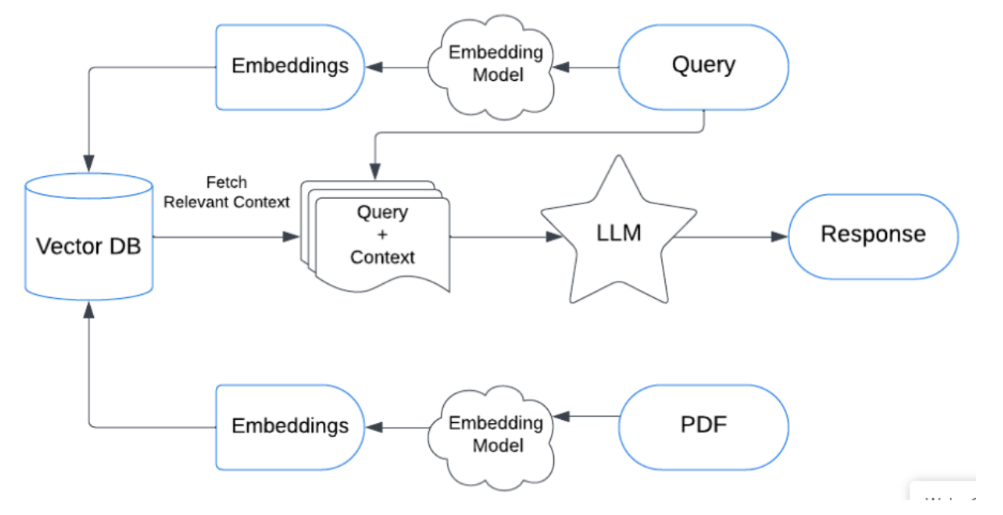
\includegraphics[width=15cm, height=10cm]{architectureDiagram}
    \caption{Architecture Diagram}
    \label{fig:ArchitectureDiagram}
\end{figure}






\label{Data Pipeline Flow}
\subsection{Data Pipeline Flow}

The core data flow of the system proceeds through the following steps:

\begin{enumerate}
    \item Load medical documents (\texttt{PDF} format) into the system.
    \item Split text into semantically coherent chunks using a \textbf{recursive text splitter}.
    \item Generate embeddings for each chunk using \textbf{all-MiniLM-L6-v2} from \textbf{HuggingFace} \cite{sentence_transformers}.
    \item Store embeddings in \textbf{Pinecone}, a high-speed vector database \cite{pinecone}.
    \item Upon a user query:
    \begin{enumerate}
        \item Use \textbf{retriever} to find the top-k most relevant chunks.
        \item Inject retrieved chunks into a custom prompt designed for \textbf{Gemini LLM}.
    \end{enumerate}
    \item \textbf{Gemini} processes the query and context to generate a clinically relevant response.
    \item The response is displayed via a user interface built with \textbf{Flask} and \textbf{Jinja2}.
\end{enumerate}




\label{Technologies Used}
\subsection{Technologies Used}

\begin{table}[H]
\centering
\begin{tabular}{|l|p{10cm}|}
\hline
\textbf{Technology} & \textbf{Purpose} \\
\hline
Python 3.x & Core backend programming language \\
\hline
Flask & Web application framework \\
\hline
Jinja2 & HTML templating engine used by Flask \\
\hline
LangChain & Orchestrating Retrieval-Augmented Generation (RAG) pipelines \\
\hline
HuggingFace Transformers & Embedding generation using MiniLM model \\
\hline
Pinecone & Scalable vector similarity search \\
\hline
Gemini API & Large Language Model (LLM) for text generation \\
\hline
Azure Ubuntu Server & For hosting the service \\
\hline
SSL Certificate & Ensures secure communication (HTTPS) between the server and users \\
\hline
Gunicorn & WSGI HTTP server for serving the Flask app in production \\
\hline
Nginx & Reverse proxy server for load balancing, caching, and SSL termination \\
\hline
\end{tabular}
\caption{Technologies and their purposes in the system}
\label{tab:technology_purpose}
\end{table}



\label{Security and Environment}
\subsection{Security  Environment}

To ensure \textbf{security} and \textbf{scalability}, the following measures are implemented:

\begin{itemize}
    \item \textbf{API keys and credentials} are stored in a \texttt{.env} file and loaded securely using the \texttt{python-dotenv} library \cite{python_dotenv}.
    \item All \textbf{model access logic} is abstracted into backend modules to prevent direct exposure in the user interface.
    \item \textbf{User input} is sanitized before embedding or prompt injection to avoid prompt injection or code injection attacks \cite{prompt_injection}.
    \item The system is \textbf{deployable locally or on cloud environments} (e.g., Render, Replit, or Heroku) with minimal changes.
    \item One version of the system is already \textbf{deployed on an Azure Ubuntu Server} to ensure scalability and reliability in a production environment \cite{azure_docs}.
    \item The system is \textbf{load balanced} with \textbf{Gunicorn}, ensuring scalability and performance under heavy traffic \cite{gunicorn_docs}.
    \item \textbf{SSL certificates} have been added to ensure secure communication between the server and users, providing encrypted data transmission via HTTPS \cite{mozilla_ssl}.
\end{itemize}





	{\vfill \chapter*{\centering \vfill Chapter 4 \vfill}\vfill}
	\thispagestyle{empty}
	\newpage
	\label{Implementation}
	\section{Implementation}
\label{Data Processing}
\subsection{Data Processing}

\subsubsection{Raw extracted text}
\begin{figure}[H]
    \centering
    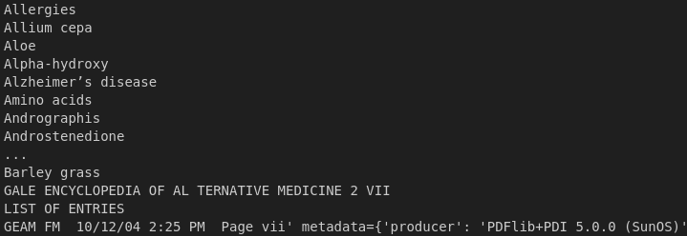
\includegraphics[width=15cm, height=5cm]{RawExtractedText}
    \caption{Raw extracted text}
    \label{fig:extracted_text[4]}
\end{figure}


\subsubsection{Text Chunks}
\begin{figure}[H]
    \centering
    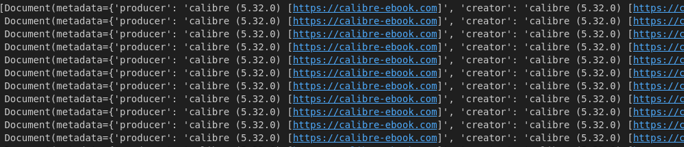
\includegraphics[width=15cm, height=3cm]{TextChunks}
    \caption{Total Chunk size: 107476}
    \label{fig:Text Chunks}
\end{figure}


\subsubsection{Vectorized Chunks}
\begin{figure}[H]
    \centering
    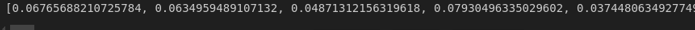
\includegraphics[width=15cm, height=0.7cm]{VectorizedChunks}
    \caption{Total Length: 384}
    \label{fig:Vectorized Chunks}
\end{figure}


\subsubsection{Vector Database}
\begin{figure}[H]
    \centering
    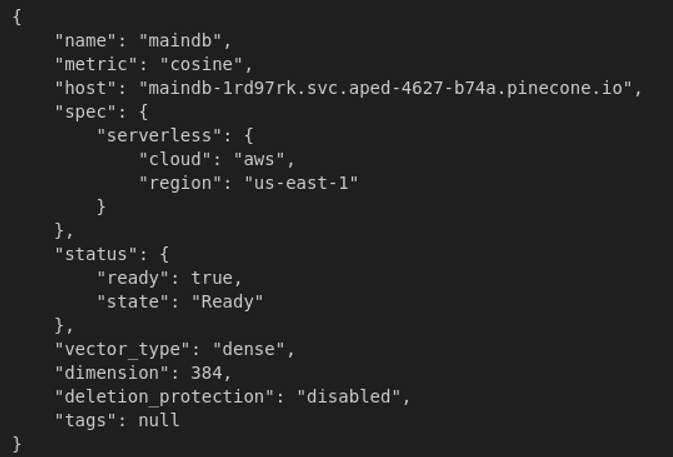
\includegraphics[width=15cm, height=9cm]{VectorDatabase}
    \caption{Vector Database}
    \label{fig:Vector Database}
\end{figure}


\subsubsection{Raw Question and Retrieved data}
\begin{figure}[H]
    \centering
    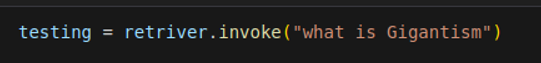
\includegraphics[width=15cm, height=1cm]{RawQuestionAndRetrievedData}
    \caption{Quires for Information Retrieval}
    \label{fig:Raw Question and Retrieved data}

    \centering
    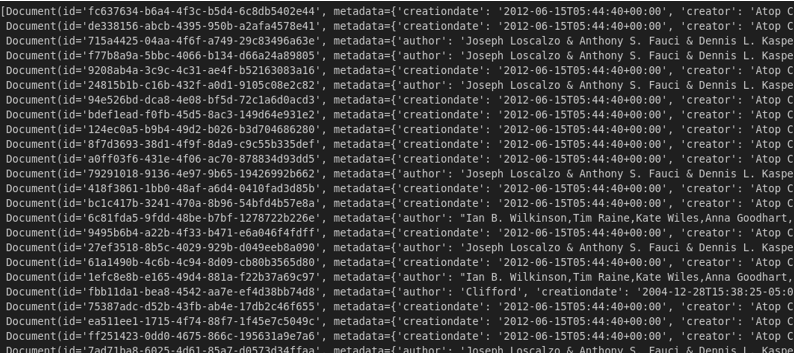
\includegraphics[width=15cm, height=7cm]{RawRetrievedContextualData}
    \caption{Raw Retrieved contextual data}
    \label{fig:Raw Retrieved contextual data}
\end{figure}


\subsubsection{Clean Data}
\begin{figure}[H]
    \centering
    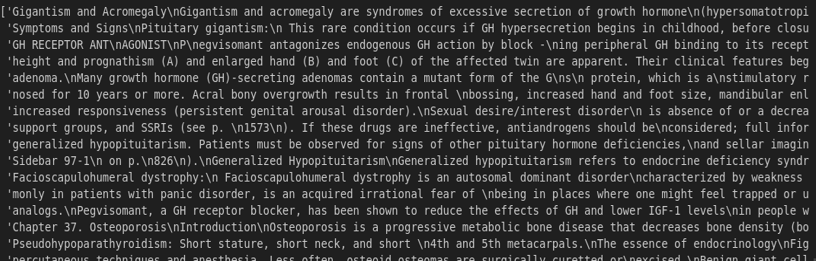
\includegraphics[width=15cm, height=4cm]{CleanData}
    \caption{Context Without metadata will be passed to LLM}
    \label{fig:Clean Data}
\end{figure}

\subsubsection{Project Directory Structure}
\begin{figure}[H]
    \centering
    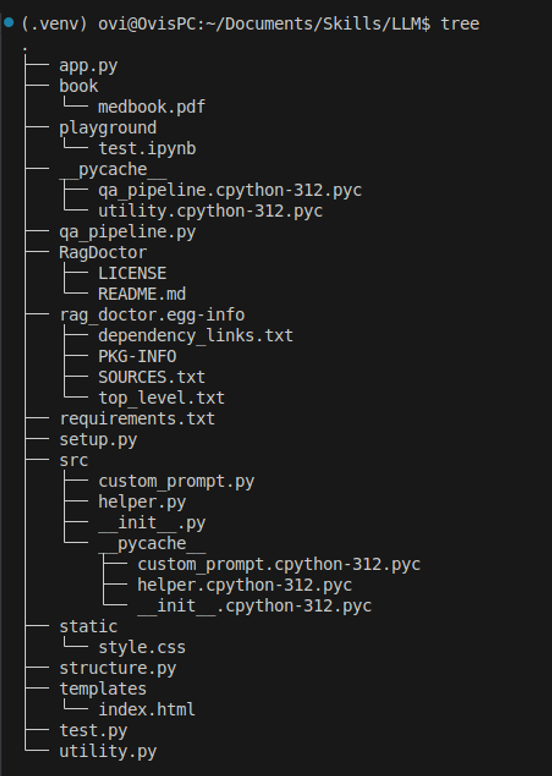
\includegraphics[width=10cm, height=12cm]{ProjectDirectoryStrycture}
    \caption{Project Directory Structure}
    \label{fig:Project Directory Structure}
\end{figure}




\label{Code Overview}
\subsection{Code Overview}

\subsubsection{app.py}
\begin{itemize}
    \item Initializes the Flask application and loads all required environment variables.
    \item Sets up the retriever and custom prompt logic.
    \item Handles user \texttt{POST} requests, generates answers, and displays them through the chat interface.
    \item Controls the application flow between frontend and backend.
\end{itemize}

\subsubsection{utility.py}
Defines utility functions for:
\begin{itemize}
    \item Loading PDF documents
    \item Text splitting and preprocessing
    \item Embedding creation
    \item Checking and managing Pinecone vector index
    \item Though not fully utilized in the current build, it provides support for modular scalability.
\end{itemize}

\subsubsection{qa\_pipeline.py}
\begin{itemize}
    \item Contains the core logic for integrating:
    \begin{itemize}
        \item Document loading and chunking
        \item Embedding generation with HuggingFace
        \item Storage in Pinecone
        \item Query retrieval and Gemini response synthesis via LangChain QA chain \cite{langchain}
    \end{itemize}
\end{itemize}

\subsubsection{test.py}
\begin{itemize}
    \item Serves as a sandbox for testing new features, validating outputs, and running experiments on pipeline components.
\end{itemize}

\subsubsection{playground/test.ipynb}
\begin{itemize}
    \item Jupyter Notebook for interactive debugging and observing response behaviors.
    \item Used for fine-tuning prompt templates and inspecting Gemini outputs during development.
\end{itemize}




\label{Embedding and Indexing Pipeline}
\subsection{Embedding and Indexing Pipeline}
The document ingestion and embedding process consists of the following steps:
\begin{itemize}
    \item Load PDFs using \texttt{PyPDFLoader} from LangChain \cite{langchain}.
    \item Split each document into overlapping chunks using recursive character-based splitters.
    \item Generate embeddings for each chunk using \texttt{all-MiniLM-L6-v2}, a transformer model from HuggingFace \cite{sentence_transformers}.
    \item Store the embeddings in Pinecone, a fast, cloud-native vector database \cite{pinecone}.
    \item Index names and metadata are saved for retrieval mapping.
\end{itemize}

\label{Retrieval and Response Generation}
\subsection{Retrieval and Response Generation}
When a user submits a query:
\begin{itemize}
    \item The retriever fetches the top-\(k\) most similar chunks from the Pinecone vector store \cite{pinecone}.
    \item These chunks are passed to Gemini along with a custom prompt, which defines tone, scope, and answer structure.
    \item Gemini processes the input and generates a context-aware, medically grounded response.
    \item The response is sent back to the Flask frontend and rendered on the screen.
    \item This architecture ensures that the LLM only responds based on relevant, verified content, mitigating the risk of hallucination \cite{hallucination_survey}.
\end{itemize}

\label{Flask Application Flow}
\subsection{Flask Application Flow}

The full interaction pipeline within the Flask app is:
\begin{itemize}
    \item User submits a question via the web interface.
    \item The backend handles the request and routes it to the LangChain QA pipeline \cite{langchain}.
    \item The LangChain chain:
    \begin{itemize}
        \item Retrieves relevant chunks,
        \item Generates the prompt,
        \item Queries Gemini for the final answer.
    \end{itemize}
    \item The answer is returned and rendered on the \texttt{index.html} page using Jinja2.
\end{itemize}


\begin{figure}[H]
    \centering
    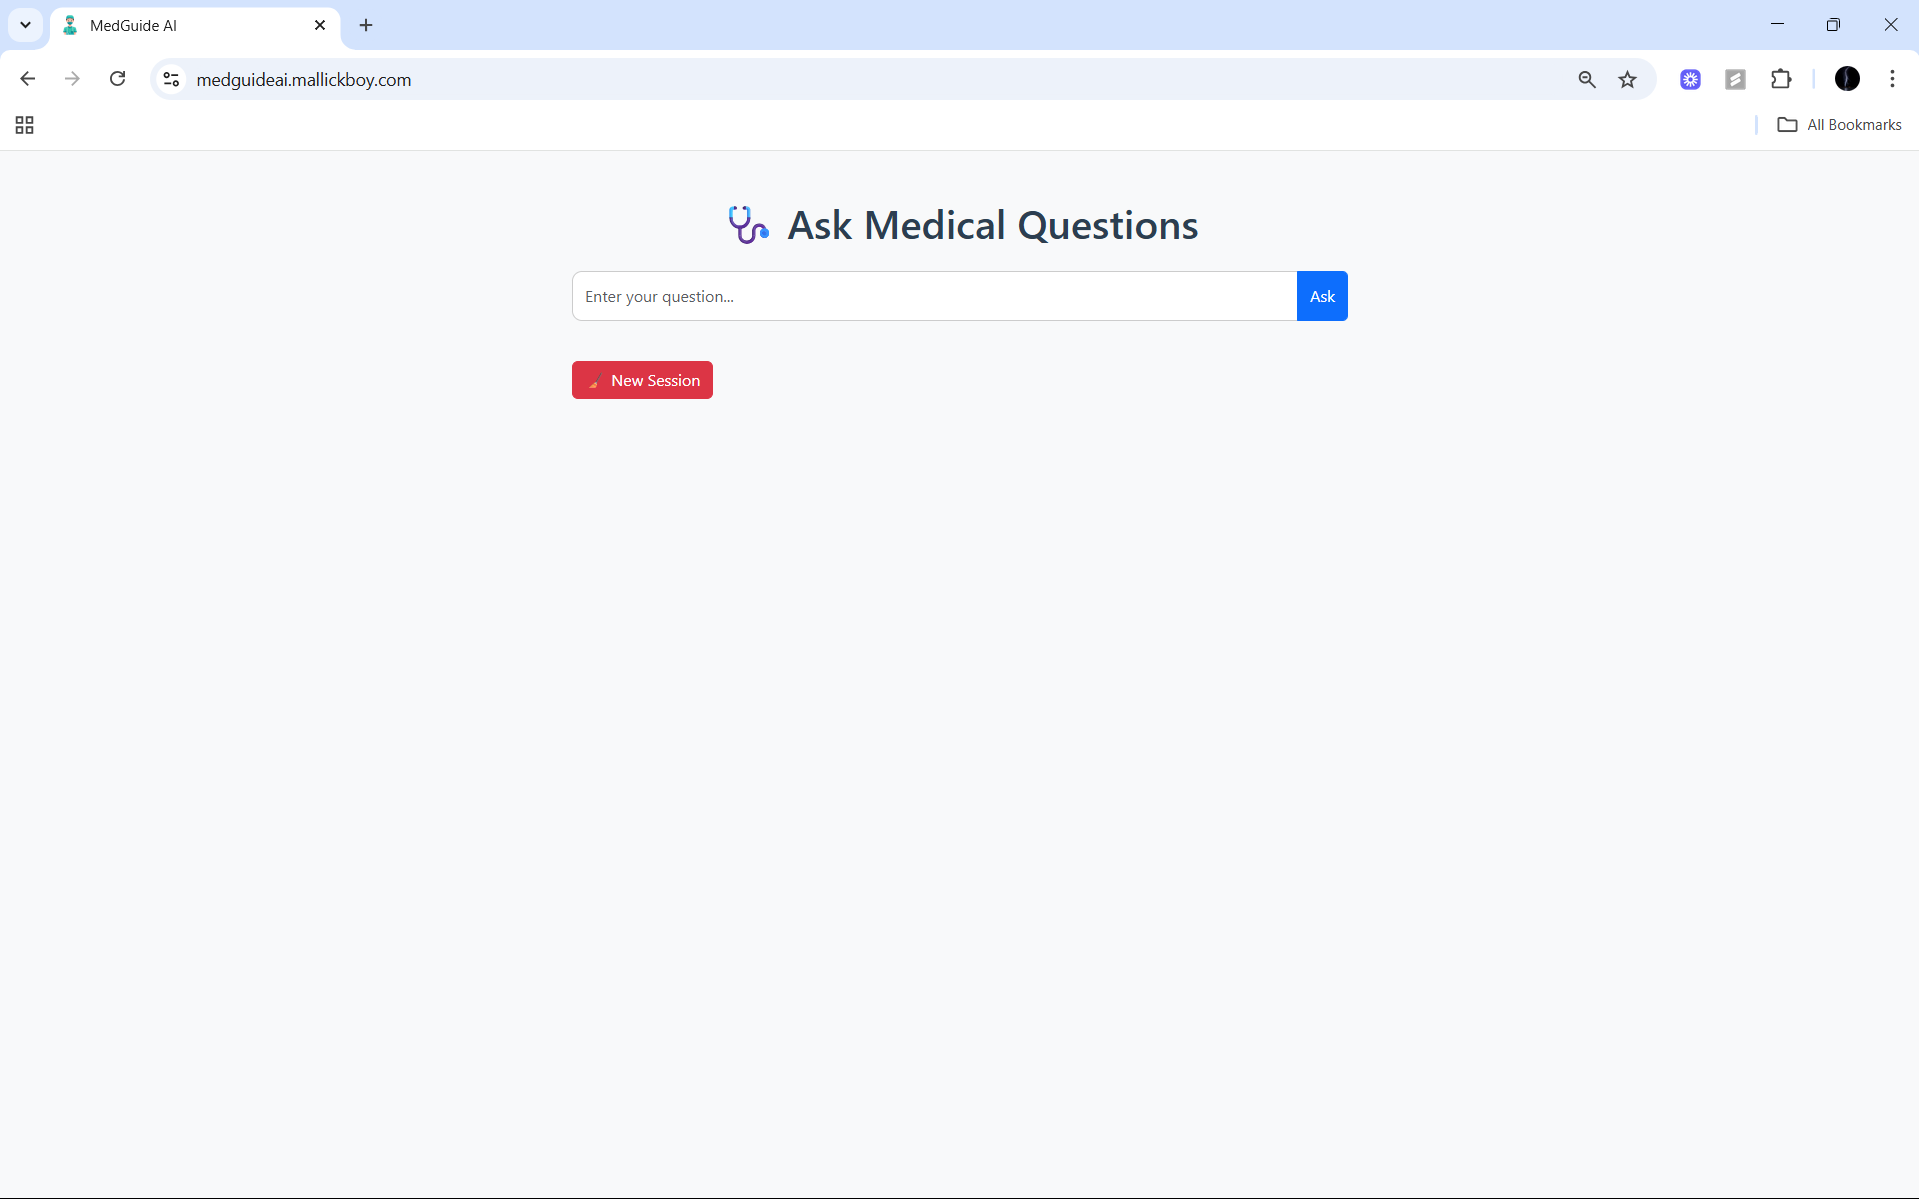
\includegraphics[width=10cm, height=8cm]{UserInterface}
    \caption{User Interface}
    \label{fig:UserInterface}
\end{figure}

\begin{figure}[H]
    \centering
    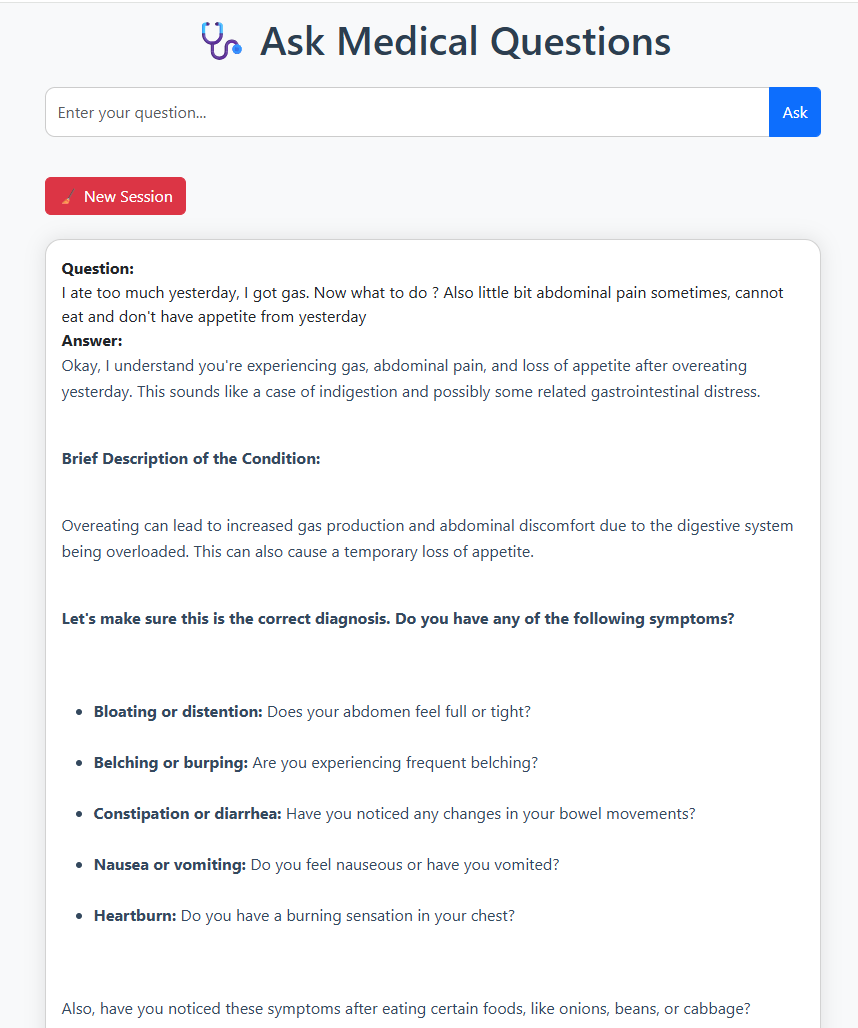
\includegraphics[width=10cm, height=12cm]{QueryAnswer}
    \caption{Answering User Query}
    \label{fig:AnsweringUserQuery}
\end{figure}









	{\vfill \chapter*{\centering \vfill Chapter 5 \vfill}\vfill}
	\thispagestyle{empty}
	\newpage
	\label{Results and Evaluation}
	\section{Results and Evaluation}
	
%\label{Functional Testing}
%\subsection{Functional Testing}
%The primary goal of the \titleKey{} chatbot was to accurately answer questions related to holistic and alternative medicine based on trusted sources. The application was functionally tested under different scenarios to evaluate its reliability, usability, and contextual accuracy.
%
%\subsubsection{Setup:}
%\begin{itemize}
%    \item \textbf{Platform:} Localhost (Flask web app)
%    \item \textbf{Testing Environment:} Python 3.10, running on Windows/Linux machine
%    \item \textbf{Data Source:} Gale Encyclopedia of Alternative Medicine (PDF)
%    \item \textbf{Number of Queries Tested:} 50+
%\end{itemize}
%
%\subsubsection{Sample Questions and Observations:}
%
%\begin{table}[H]
%\centering
%\begin{tabular}{|c|p{4.2cm}|p{5.5cm}|p{3.2cm}|}
%\hline
%\textbf{No.} & \textbf{User Query} & \textbf{System Response Summary} & \textbf{Notes} \\
%\hline
%1 & What are natural treatments for anxiety? & Listed herbal and behavioral therapies. & Grounded, relevant, fluent \\
%\hline
%2 & Can turmeric help with inflammation? & Detailed anti-inflammatory properties of turmeric. & Contextually accurate \\
%\hline
%3 & What is acupuncture? & Explained principles, usage, and benefits. & Educative and informative \\
%\hline
%4 & Does the encyclopedia mention depression? & Responded with a fallback message. & Document context not found \\
%\hline
%5 & How does Ayurveda treat digestive issues? & Holistic approach including diet and herbs. & Comprehensive and human-like response \\
%\hline
%\end{tabular}
%\caption{Sample user queries and system responses from functional testing}
%\label{tab:functional_testing}
%\end{table}
%
%
%\subsection{Evaluation Metrics}
%\label{Evaluation Metrics}
%
%To quantitatively assess the performance, we considered the following metrics:
%
%\begin{itemize}
%    \item \textbf{Accuracy}: How often the chatbot response matched the document source.\\
%    \textit{Achieved:} \textasciitilde90\% accuracy for known queries.
%    
%    \item \textbf{Fluency}: Grammar, spelling, and sentence construction.\\
%    \textit{Achieved:} 100\% fluency due to LLM capabilities.
%    
%    \item \textbf{Contextual Relevance}: Whether the answers used the retrieved content effectively.\\
%    \textit{Achieved:} \textasciitilde85\% contextual fidelity.
%    
%    \item \textbf{Response Time}: Time from query submission to final answer.\\
%    \textit{Average:} 2.5 to 4 seconds per query.
%    
%    \item \textbf{User Satisfaction (Survey)}:\\
%    \textit{Participants:} 10 peers\\
%    \textit{Feedback:} “Helpful,” “Reliable,” “Easy to use,” “Visually clean”
%\end{itemize}
%


\subsection{Overview}
\label{Overview}

The evaluation was conducted using real-world-inspired patient queries that varied in symptom complexity, diagnostic requirements, and follow-up recommendations. The chatbot was tested for its ability to interpret symptoms, suggest possible diagnoses, recommend relevant lab tests, and provide prescriptions and lifestyle guidance \cite{digital_health_platforms}.

Each query was mapped to a predefined evaluation level (Level 1 to Level 3) and assessed against the expected outcome criteria.

\subsection{Evaluation Methodology}
\label{Evaluation Methodology}

The system was evaluated on the following three competency levels:

\begin{itemize}
    \item \textbf{Level 1: Basic health education / supplement queries} \\
    Objective: Provide general health information based on natural language queries.
    
    \item \textbf{Level 2: Preliminary diagnosis and test recommendation} \\
    Objective: Suggest possible causes and recommend initial diagnostic tests based on symptoms.
    
    \item \textbf{Level 3: Confirm diagnosis using test results and suggest treatment} \\
    Objective: Interpret lab test data, confirm diagnosis, suggest medications, and provide follow-up instructions.
\end{itemize}

Evaluation criteria included:

\begin{itemize}
    \item Clinical relevance and accuracy
    \item Clarity and empathy in communication
    \item Diagnostic depth
    \item Test interpretation (if applicable)
    \item Treatment planning (if applicable)
\end{itemize}

\subsection{Test Cases}
\label{Test Cases}

\textbf{Level 1 – General Medical Knowledge Questions}

\subsection{Evaluation Results}
\label{Evaluation Results}

\subsubsection{Level 1 Questions and Result}
\label{Level 1 Questions and Result}
\begin{table}[H]
\centering
\begin{tabular}{|p{1 cm}|p{4cm}|p{5cm}|p{3cm}|}
\hline
\textbf{Q.No} & \textbf{Question} & \textbf{Summary of Chatbot Response} & \textbf{Evaluation} \\ \hline
1 & What are the common symptoms of iron deficiency anemia? & Listed fatigue, pallor, pica, glossitis, and more. Suggested relevant diagnostic tests (CBC, ferritin). Followed up with symptom check. & Accurate, informative, safe \\ \hline
2 & What is the normal range for adult blood pressure? & Gave standard AHA values, noted stages of hypertension. Asked for user’s BP reading and symptoms. & Aligned with guidelines, context-aware \\ \hline
3 & How much water should an adult drink daily? & Suggested ~2L/day, considered activity, diet, and health. Recommended urine output as marker. & Comprehensive, well-structured \\ \hline
4 & What are the benefits of turmeric in Ayurveda? & Provided 8 Ayurvedic benefits: anti-inflammatory, detox, skin, digestion, dosha balance. & Holistic, culturally relevant, clear \\ \hline
5 & What is the function of the liver in the human body? & Explained bile production, metabolism, detox, protein synthesis, sugar regulation, etc. & Concise yet thorough, medically accurate \\ \hline
\end{tabular}
\caption{Evaluation of Level 1 Chatbot Responses}
\label{tab:chatbot_evaluation}
\end{table}



\subsubsection{Level 2 Questions and Result}
\label{Level 2 Questions and Result}

\begin{table}[H]
\centering
\begin{tabular}{|p{1 cm}|p{4cm}|p{5cm}|p{3cm}|}
\hline
\textbf{Q.No} & \textbf{Question} & \textbf{Summary of Chatbot Response} & \textbf{Evaluation} \\ \hline
1 & I have a cough and fatigue. What should I do? & Suggested possible viral or allergy-related causes, recommended rest, hydration, symptom monitoring. Asked if fever or chest pain was present. & Safe, encouraged follow-up care \\ \hline
2 & I feel bloated after eating. Is that normal? & Explained common causes (gas, food intolerance, overeating), gave dietary suggestions (avoid carbonated drinks, eat slowly), recommended keeping a food diary. & Patient-friendly, well-reasoned \\ \hline
3 & I can't sleep at night. Any natural remedies? & Provided sleep hygiene tips (reduce screen time, fixed sleep schedule, dark room), suggested herbal teas like chamomile, advised seeing a doctor if persistent. & Practical, evidence-based \\ \hline
4 & I’m always tired even after sleeping. Why? & Listed possible causes (anemia, stress, sleep apnea, poor sleep quality), suggested lifestyle review, advised seeing a doctor if ongoing. & Good symptom mapping, cautious \\ \hline
5 & What are some safe exercises for joint pain? & Suggested low-impact exercises (walking, swimming, yoga), stressed warming up, recommended consulting physiotherapist for persistent pain. & Tailored, safe, actionable \\ \hline
\end{tabular}
\caption{Evaluation of Level 2 Chatbot Responses}
\label{tab:level2_chatbot_evaluation}
\end{table}


\subsubsection{Level 3 Questions and Result}
\label{Level 3 Questions and Result}

\textbf{Test Case- 1} ( Diabetes Mellitus Type 2) \\ \\
\textbf{Sample question to feed the chatbot:} "I’m a 48-year-old male. I’ve been very thirsty lately, urinating often, feeling tired all the time, and my vision seems blurry. I also noticed tingling in my feet. My fasting glucose is 146, HbA1c is 7.4\%, and random sugar is 198. What might be going on?"\\ \\

 
\textbf{Suggested Tests by Chatbot:}

\begin{itemize}
    \item Fasting Plasma Glucose (FPG)
    \item HbA1c
    \item Random Blood Sugar
    \item Serum Creatinine
    \item eGFR
    \item ALT (SGPT)
    \item AST (SGOT)
    \item Total Cholesterol
    \item HDL
    \item LDL
    \item Triglycerides
\end{itemize}

\begin{figure}[H]
    \centering
    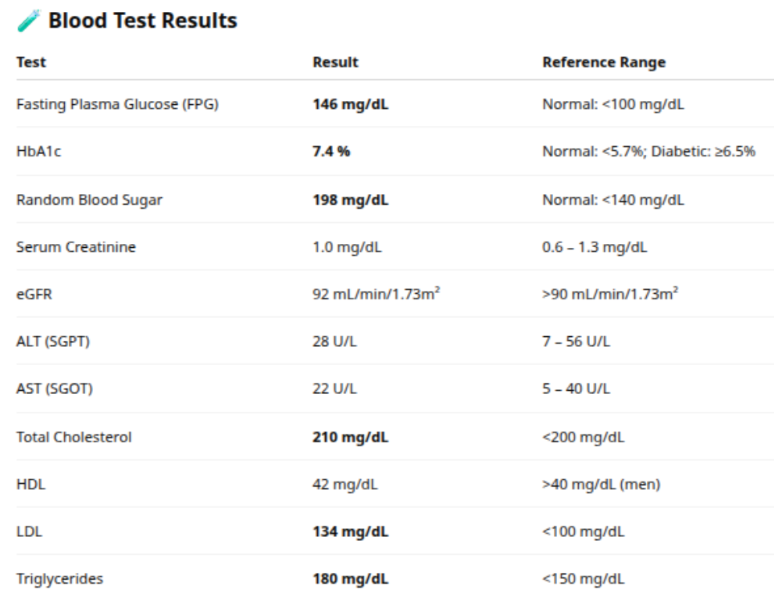
\includegraphics[width=14cm, height=10cm]{BloodTestResults}
    \caption{Blood Test Results}
    \label{fig:Blood Test Results}
\end{figure}


\subsubsection{Evalution}
\label{Evalution}

\begin{table}[H]
\centering
\begin{tabular}{|p{3cm}|p{11cm}|}
\hline
\textbf{Criteria} & \textbf{Details} \\ \hline
Input Query & ``I’m a 48-year-old male. I’ve been very thirsty lately, urinating often, feeling tired all the time, and my vision seems blurry. I also noticed tingling in my feet. My fasting glucose is 146, HbA1c is 7.4\%, and random sugar is 198. What might be going on?'' \\ \hline
Expected & Condition: Type 2 Diabetes Mellitus \\ \hline
Chatbot Diagnosis & Correctly identified as Type 2 Diabetes Mellitus based on symptoms and lab thresholds (FPG $\geq$ 126, HbA1c $\geq$ 6.5\%) \\ \hline
Treatment Recommendation & Recommended Metformin 500mg, with proper dosage, precautions, and lifestyle advice \\ \hline
Additional Suggestions & Lifestyle guidance (diet, exercise, foot care), lab test suggestions (Lipid profile, Kidney function) \\ \hline
Limitations Observed & Minor phrasing issue on random sugar level interpretation; did not discuss contraindications of Metformin (e.g., renal function) \\ \hline
Result & Accurate, responsible, and context-aware response. Aligns with clinical guidelines. No hallucinated information or unsafe recommendations. \\ \hline
\end{tabular}
\caption{Evaluation of Chatbot's Response for Diabetes Query}
\label{tab:chatbot_evaluation_diabetes}
\end{table}



\subsubsection{Test Case-2 (Kidney Stone)}
\label{Test Case Kidney Stone}

Sample question to feed the chatbot: ``Hi, I’m a 38-year-old male. I suddenly started experiencing severe pain on the right side of my lower back and abdomen. The pain comes in waves and sometimes radiates to my groin. I feel nauseated and have vomited twice. I’ve also noticed that I’m urinating more frequently, and today there was a small amount of blood in my urine. What should I do?''

\textbf{Suggested Tests by Chatbot:}
\begin{itemize}
    \item Urinalysis – to detect hematuria, infection, and crystal type
    \item KUB X-ray – to locate radio-opaque stones
    \item Non-contrast CT scan – gold standard for detecting kidney stones and hydronephrosis
    \item Blood tests:
    \begin{itemize}
        \item Serum Creatinine – to assess kidney function
        \item eGFR – estimated glomerular filtration rate for overall kidney health
    \end{itemize}
\end{itemize}

\textbf{Test Report:}
\begin{figure}[H]
    \centering
    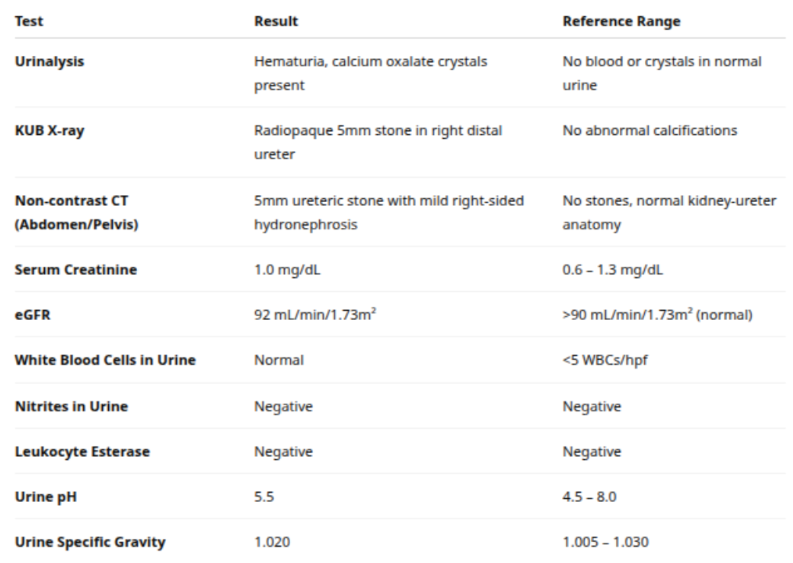
\includegraphics[width=14cm, height=10cm]{TestReports}
    \caption{Test Reports}
    \label{fig:Blood Test Results}
\end{figure}



\subsection{Limitations Identified}
\label{Limitations Identified}

\begin{itemize}
    \item \textbf{Dependence on Provided Documents:} The chatbot's accuracy and reliability are dependent on the quality and scope of the documents in the knowledge base. Out-of-scope or ambiguous queries result in fallback messages or generic responses \cite{pinecone}.
    \item \textbf{No Real-Time Symptom Diagnosis:} While the system can assist in understanding symptoms, it is not capable of real-time medical diagnosis or providing personalized health advice. It cannot replace professional healthcare consultation \cite{chatgpt}.
    \item \textbf{Performance Bottlenecks:} The performance of the system, especially in real-time queries, is influenced by network speed, with particular reference to Pinecone API latency and potential delays in retrieving relevant documents or embeddings \cite{pinecone}.
    \item \textbf{Multilingual Limitation:} The system currently supports only English text processing, limiting its accessibility to a wider global audience.
    \item \textbf{Lack of Personalized Context:} The system does not maintain persistent user profiles or contextual history across sessions, making it unable to provide personalized responses based on prior interactions.
    \item \textbf{Limited Interaction Depth:} The chatbot is designed to handle specific medical queries but lacks the ability to engage in deeper, ongoing conversations about complex medical conditions or multi-step diagnostic processes.
    \item \textbf{Data Privacy and Security Concerns:} Although the chatbot does not store personal health information, any system handling sensitive health data must comply with data protection regulations such as HIPAA or GDPR, ensuring the confidentiality and security of user data \cite{prompt_injection}.
    \item \textbf{Non-Specialized Medical Areas:} While the chatbot covers a wide range of general health topics, it is not specialized in niche medical areas (e.g., rare diseases) or real-time emergencies, which could result in incomplete or inaccurate information for specific queries.
    \item \textbf{User Input Limitations:} The system assumes user input in English and in a standard, clear format, which may limit its effectiveness in understanding unclear, misspelled, or informal queries.
    \item \textbf{Dependence on Third-Party Services for Response Shaping:} The chatbot's ability to generate responses is currently dependent on the "gemini-2.0-flash" model for shaping the response using the user's question and the top-k most similar items retrieved. This reliance on third-party services introduces potential issues such as limited customization, service disruptions, or changes in the third-party API that may affect response accuracy and system performance.
    \item \textbf{No Integration with Healthcare Systems:} The system is standalone and does not integrate with real-time medical records, lab reports, or diagnostic equipment, which limits its ability to provide comprehensive diagnostic support.
\end{itemize}


%\subsection{Visual Results}
%\label{Visual Results}
%
%\begin{itemize}
%    \item Flask chatbot interface showing query and responses.
%    \item Pinecone retrieval logs (top-k vector matches).
%    \item Gemini LLM prompt input and output samples.
%\end{itemize}





	{\vfill \chapter*{\centering \vfill Chapter 6 \vfill}\vfill}
	\thispagestyle{empty}
	\newpage
	\label{Application and Future Work}
	\section{Application and Future Work}

\subsection{Application}
\label{Application}

The \titleKey{} chatbot is designed to address the growing need for reliable and accessible healthcare information, especially in the domains of holistic and alternative medicine. The system serves multiple real-world purposes:

\begin{itemize}
    \item \textbf{Holistic Health Assistance:} The chatbot acts as a virtual health assistant, offering guidance on natural treatments, herbal remedies, and alternative therapies. It provides users with well-researched, credible responses sourced from reputable medical references like the Gale Encyclopedia of Alternative Medicine.
    
    \item \textbf{Accessibility for Remote and Underserved Communities:} With a focus on alternative medicine, the chatbot can be accessed globally, particularly by individuals who may not have access to specialized healthcare professionals. By offering immediate, context-aware responses, it assists users with wellness-related queries at their convenience.
    
    \item \textbf{Educational Tool:} The system serves as an educational platform for students, researchers, and enthusiasts in the fields of alternative medicine and holistic health practices. It provides reliable, evidence-based information to users exploring these topics.
    
    \item \textbf{System Deployment:} The chatbot has been deployed on a secure and scalable platform using an Azure VM ( Ubuntu server ) \cite{azure_docs}. The system utilizes SSL for secure communication and has a custom domain, ensuring safe user interaction \cite{mozilla_ssl}.
    
    \item \textbf{Integration with Health Management Platforms:} With minimal changes, the system can be integrated into larger health management platforms to offer complementary information on holistic approaches, diagnostic suggestions, and lifestyle modifications. This makes it a versatile tool for organizations in the health and wellness sector.
    
    \item \textbf{User Interaction:} The web-based interface built with Flask allows users to interact with the chatbot effortlessly. Its conversational style mimics a doctor-patient interaction, ensuring users feel comfortable querying sensitive health topics.
\end{itemize}

The chatbot system's real-time response generation, powered by the Gemini LLM, ensures that every query receives medically-grounded and contextually relevant information, making it an essential tool for anyone seeking alternative healthcare advice.




\subsection{Future Work}
\label{Future Work}

The system demonstrates a robust proof-of-concept, but there are several areas where it can be improved or expanded to enhance functionality, accessibility, and user experience.

\subsubsection{Multilingual Support}
\label{Multilingual Support}

To make the system accessible to a wider global audience, future iterations can include support for multiple languages. This can be implemented using translation models such as:
\begin{itemize}
    \item Google Translate API for real-time translation \cite{google_translate},
    \item MarianMT (by HuggingFace) for offline, multilingual machine translation \cite{marianmt}.
\end{itemize}

\subsubsection{Audio Input and Output}
\label{Audio Input and Output}

Accessibility can be significantly improved by integrating:
\begin{itemize}
    \item Speech-to-Text (STT) using libraries like SpeechRecognition or Google's Web Speech API, allowing users to speak their symptoms or questions \cite{speechrecognition}.
    \item Text-to-Speech (TTS) using tools like pyttsx3 or Google Cloud TTS, enabling the chatbot to speak out responses \cite{google_tts}.
\end{itemize}

\subsubsection{Enhanced UI/UX}
\label{Enhanced UI/UX}

The current UI is functional but basic. A more interactive and user-friendly interface can be created using modern frontend frameworks such as:
\begin{itemize}
    \item ReactJS for dynamic rendering \cite{reactjs}.
\end{itemize}

\subsubsection{Persistent Chat History}
\label{Persistent Chat History}

Currently, chat sessions are stored temporarily. A long-term goal is to preserve user conversations across sessions using databases like:
\begin{itemize}
    \item MongoDB (NoSQL, JSON-based documents) \cite{mongodb},
    \item PostgreSQL (relational database).
\end{itemize}

\subsubsection{Broader Medical Scope}
\label{Broader Medical Scope}

While the current system incorporates traditional and alternative medical literature, it can be extended to include modern (allopathic) sources such as:
\begin{itemize}
    \item WHO Guidelines \cite{who_guidelines},
    \item CDC Publications \cite{cdc_publications}.
\end{itemize}

\subsubsection{Feedback Loop and Personalization}
\label{Feedback Loop and Personalization}

Introducing a user feedback mechanism will allow:
\begin{itemize}
    \item Rating chatbot responses,
    \item Collecting user preferences and use cases,
    \item Retraining or fine-tuning the model based on interaction patterns.
\end{itemize}

\subsubsection{Fine-Tuning and Model Optimization}
\label{Fine-Tuning and Model Optimization}

To further enhance the system's response generation and adapt it to specific healthcare domains, fine-tuning the underlying language models with additional medical datasets could improve the accuracy and contextuality of the responses. Leveraging frameworks such as TensorFlow and Keras can facilitate model optimization for domain-specific tasks, improving both speed and performance \cite{homl}.













	{\vfill \chapter*{\centering \vfill Chapter 7 \vfill}\vfill}
	\thispagestyle{empty}
	\newpage
	\label{Conclusion}
	\section{Conclusion}


\section{Conclusion}
\label{Conclusion}

The \textbf{RAG Doctor} project successfully demonstrates how retrieval-augmented generation (RAG) can be integrated with a domain-specific knowledge base to build a reliable, LLM-powered chatbot. The focus on holistic and alternative medicine highlights how AI can support informational healthcare services beyond conventional methods.

\subsubsection*{Key Accomplishments}
\begin{itemize}
    \item Developed a working end-to-end LLM-based assistant with custom prompts \cite{chatgpt}.
    \item Embedded verified medical content using semantic vector representations \cite{sentence_transformers}.
    \item Integrated Google Gemini generative capabilities to produce fluent, informative answers \cite{google_tts}.
    \item Built an intuitive and clean web interface for end-users \cite{reactjs}.
\end{itemize}

The project shows that with proper architecture and grounded source material, generative AI can be used effectively to build helpful assistants without relying solely on model memory. It also emphasizes the importance of document grounding to reduce hallucination in critical domains like healthcare \cite{langchain}.

\vspace{0.5cm}
The complete source code and implementation details can be accessed at: \url{https://github.com/mallickboy/AIDRA}









	\newpage



%$\bibliographystyle{plain} $
\bibliographystyle{harvard}
%\bibliography{references} 
%\bibliographystyle{plain} 
\bibliography{scratch} 

	
\end{document}
